\documentclass[a4j]{jarticle}
\usepackage[dvipdfmx]{graphicx}
\usepackage[dvipdfmx]{color}
\usepackage{url}
\usepackage{here}

\begin{document}

\subsubsection{設定}
図\ref{configuration}は設定画面を示します。\\
設定では、管理者への問い合わせやアカウントの設定をすることができます。

\begin{figure}[H]
    \begin{center}
    \resizebox{8cm}{!}{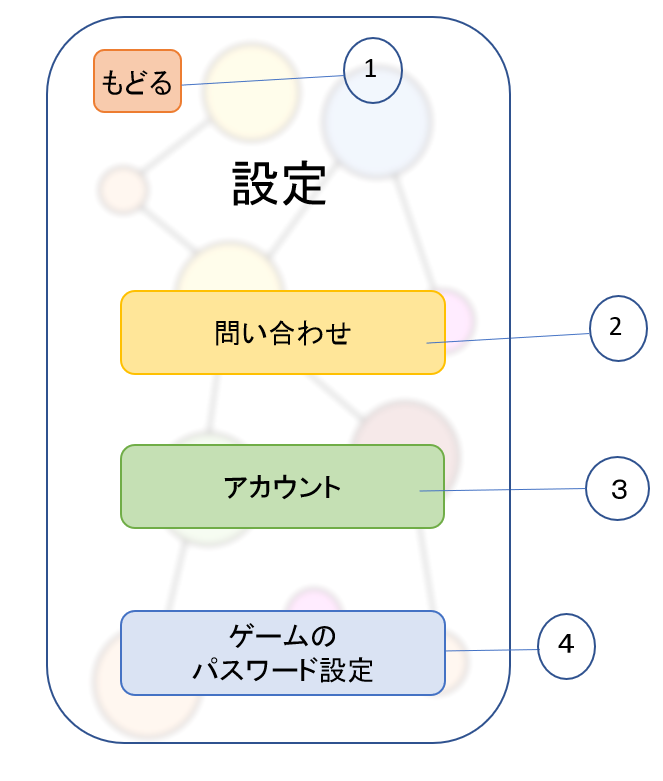
\includegraphics {configuration.png}}
    \caption {設定画面}
    \label{configuration}
    \end{center}
\end{figure}

\begin{enumerate}
  \renewcommand{\labelenumi}{\textcircled{\scriptsize \theenumi}}
\item 問い合わせ\\
  問い合わせをタップすることで問い合わせのメールアドレスと問い合わせに必要な情報を記載したページ(図\ref{inquiry})に遷移します。
\item アカウント\\
  アカウントをタップすると変更と削除の画面(図\ref{account})に遷移します。
\end{enumerate}

\begin{figure}[H]
    \begin{center}
    \resizebox{8cm}{!}{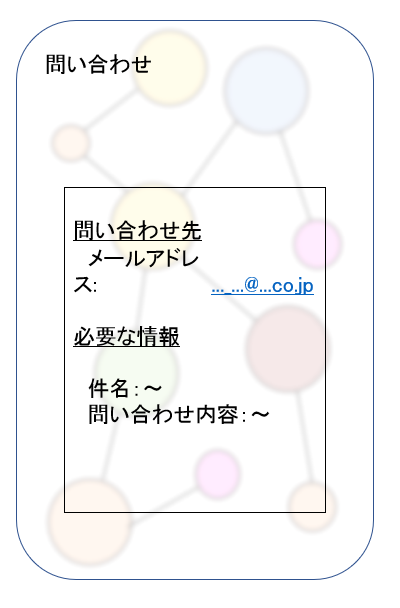
\includegraphics {inquiry.png}}
    \caption {問い合わせ}
    \label{inquiry}
    \end{center}
\end{figure}

\subsubsection{アカウント}
図\ref{account}はアカウントの設定画面を示します。\\
アカウントの設定ではアカウントの変更と削除ができます。

\begin{figure}[H]
    \begin{center}
    \resizebox{8cm}{!}{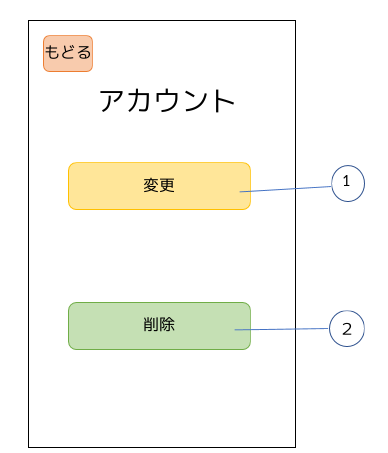
\includegraphics {account.png}}
    \caption {アカウント}
    \label{account}
    \end{center}
\end{figure}

\begin{enumerate}
  \renewcommand{\labelenumi}{\textcircled{\scriptsize \theenumi}}
\item 変更\\
  変更をタップするとニックネームと地域の設定画面(図\ref{change})に遷移します。
\item 削除\\
  削除をタップすると削除をするか確認する画面に遷移します。いいえをタップするとアカウントの設定画面(図\ref{account})に遷移します。はいをタップすると削除が完了し、確認画面(図\ref{check})へ遷移します。
\end{enumerate}

\begin{figure}[H]
    \begin{center}
    \resizebox{8cm}{!}{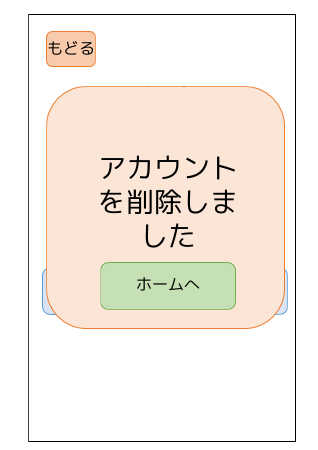
\includegraphics {check.png}}
    \caption {確認}
    \label{check}
    \end{center}
\end{figure}

\subsubsection{変更}
図\ref{change}はアカウントの変更画面を示します。\\
変更画面では、ニックネームと地域の変更ができます。

\begin{figure}[H]
  \begin{center}
    \resizebox{8cm}{!}{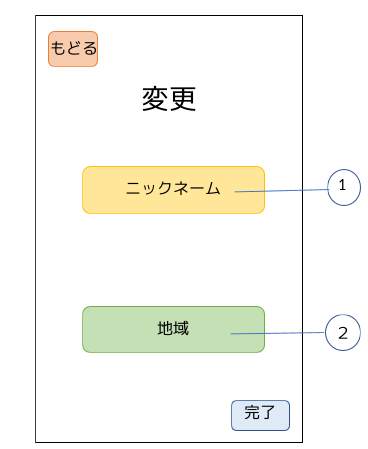
\includegraphics {change.png}}
    \caption {変更}
    \label{change}
  \end{center}
\end{figure}

\begin{enumerate}
  \renewcommand{\labelenumi}{\textcircled{\scriptsize \theenumi}}
\item ニックネーム\\
  ニックネームをタップするとキーボードが開き、入力することが可能になります。
\item 地域\\
  地域をタップすると都道府県の一覧が表示され、選択することができます。
\end{enumerate}

変更後、完了ボタンをタップすることで変更が完了します。

\end{document}
